% !TeX root = ../pythonTutorial.tex
\chapter*{Vorwort}

Das vom Stifterverband gef�rderte Projekt \glqq Informatik studieren in der digitalen Gesellschaft (InfoStuDi)\grqq{}
erprobt und evaluiert neue Lehr-, Lern- und Pr�fungsformen in den Informatik-Studieng�ngen im Fachbereich Informatik und Mikrosystemtechnik der Hochschule Kaiserslautern.

Studieng�nge an einer Hochschule f�r
angewandte Wissenschaften bereiten die Studierenden auf die sp�tere Arbeitswelt vor.
Diese Arbeitswelt
wird von zeitlich und �rtlich ungebundenem T�tigkeiten gepr�gt sein.
Im Teilprojekt \glqq Collaborative Writing\grqq{} wurde eine neue Form einer Lehrveranstaltung erprobt,
die die Studierenden auf diese sp�tere Arbeitswelt vorbereiten soll.
Ein Team aus Studierenden und Lehrenden verfasst ein Dokument zu einem Thema der Informatik.
Dabei wird neben der Produktion von Texten auch Software entstehen.
Die Produktion des vorliegenden Dokuments
zum Thema Python wurde wie ein gro�es agiles Software-Projekt organisiert.
Drei Sprints wurden durchgef�hrt, das Team organisierte sich selbst. Werkzeuge wie \LaTeX{}, Git oder Jenkins wurden eingesetzt.
Die Studierenden waren nicht nur Autoren, sondern auch Fachlektoren, Software-Entwickler und f�r die Qualit�t des Gesamtergebnisses mit verantwortlich.

Dieses Projekt w�re nicht zustande gekommen ohne die Studierenden, die sich auf dieses Abenteuer im Rahmen der Lehrveranstaltung \glqq Aktuelle Themen aus Forschung und Praxis\grqq{} des Masterstudiengangs Informatik im Wintersemester~2018/19 eingelassen haben. An dieser Stelle ein herzliches \glqq Danke sch�n!\grqq{} f�r das Vertrauen und den Mut, sich auf diese Form einer
Lehrveranstaltung einzulassen.
Miriam Lohm�ller, als wissenschaftliche Mitarbeiterin im Projekt InfoStuDi t�tig, brachte ihre Erfahrung aus dem Verlagswesen ein und hat die von den Studierenden verfassten
Texte lektoriert. Fabian Kalweit, Mitarbeiter des Projektleiters im Fachbereich Informatik und Mikrosystemtechnik, hat das fachliche Lektorat unterst�tzt und insbesondere das Backend in GitHub
organisiert und gestaltet.

Der vorliegende Text stellt den Stand im M�rz 2019, nach Abschluss der Lehrveranstaltung, dar. Nat�rlich
ist das Python-Tutorial nicht abgeschlossen. Das komplette Projekt steht in Form eines �ffentlichen Git-Repositories (\cite{githubRepo})
zur Verf�gung und kann von interessierten Studierenden verwendet und vor allem weiterentwickelt werden.
Alle Autoren hoffen, dass unsere Leser den Text f�r gut befinden.

Die Texte wurden nach bestem Wissen und
Gewissen verfasst. Sollte der Text trotzdem Fehler enthalten, liegen diese in der alleinigen Verantwortung
des Projektleiters!

\vspace{\baselineskip}
\begin{flushright}\noindent
Zweibr�cken, im Februar 2020\hfill

\hfill {\it Manfred  Brill}
\end{flushright}
\pagebreak
\section*{Das Team}
%Gruppenbild mit Dame -- das Team nach dem letzten Sprint Meeting am 31.~Januar~2019.

\begin{figure}[ht]
\centering
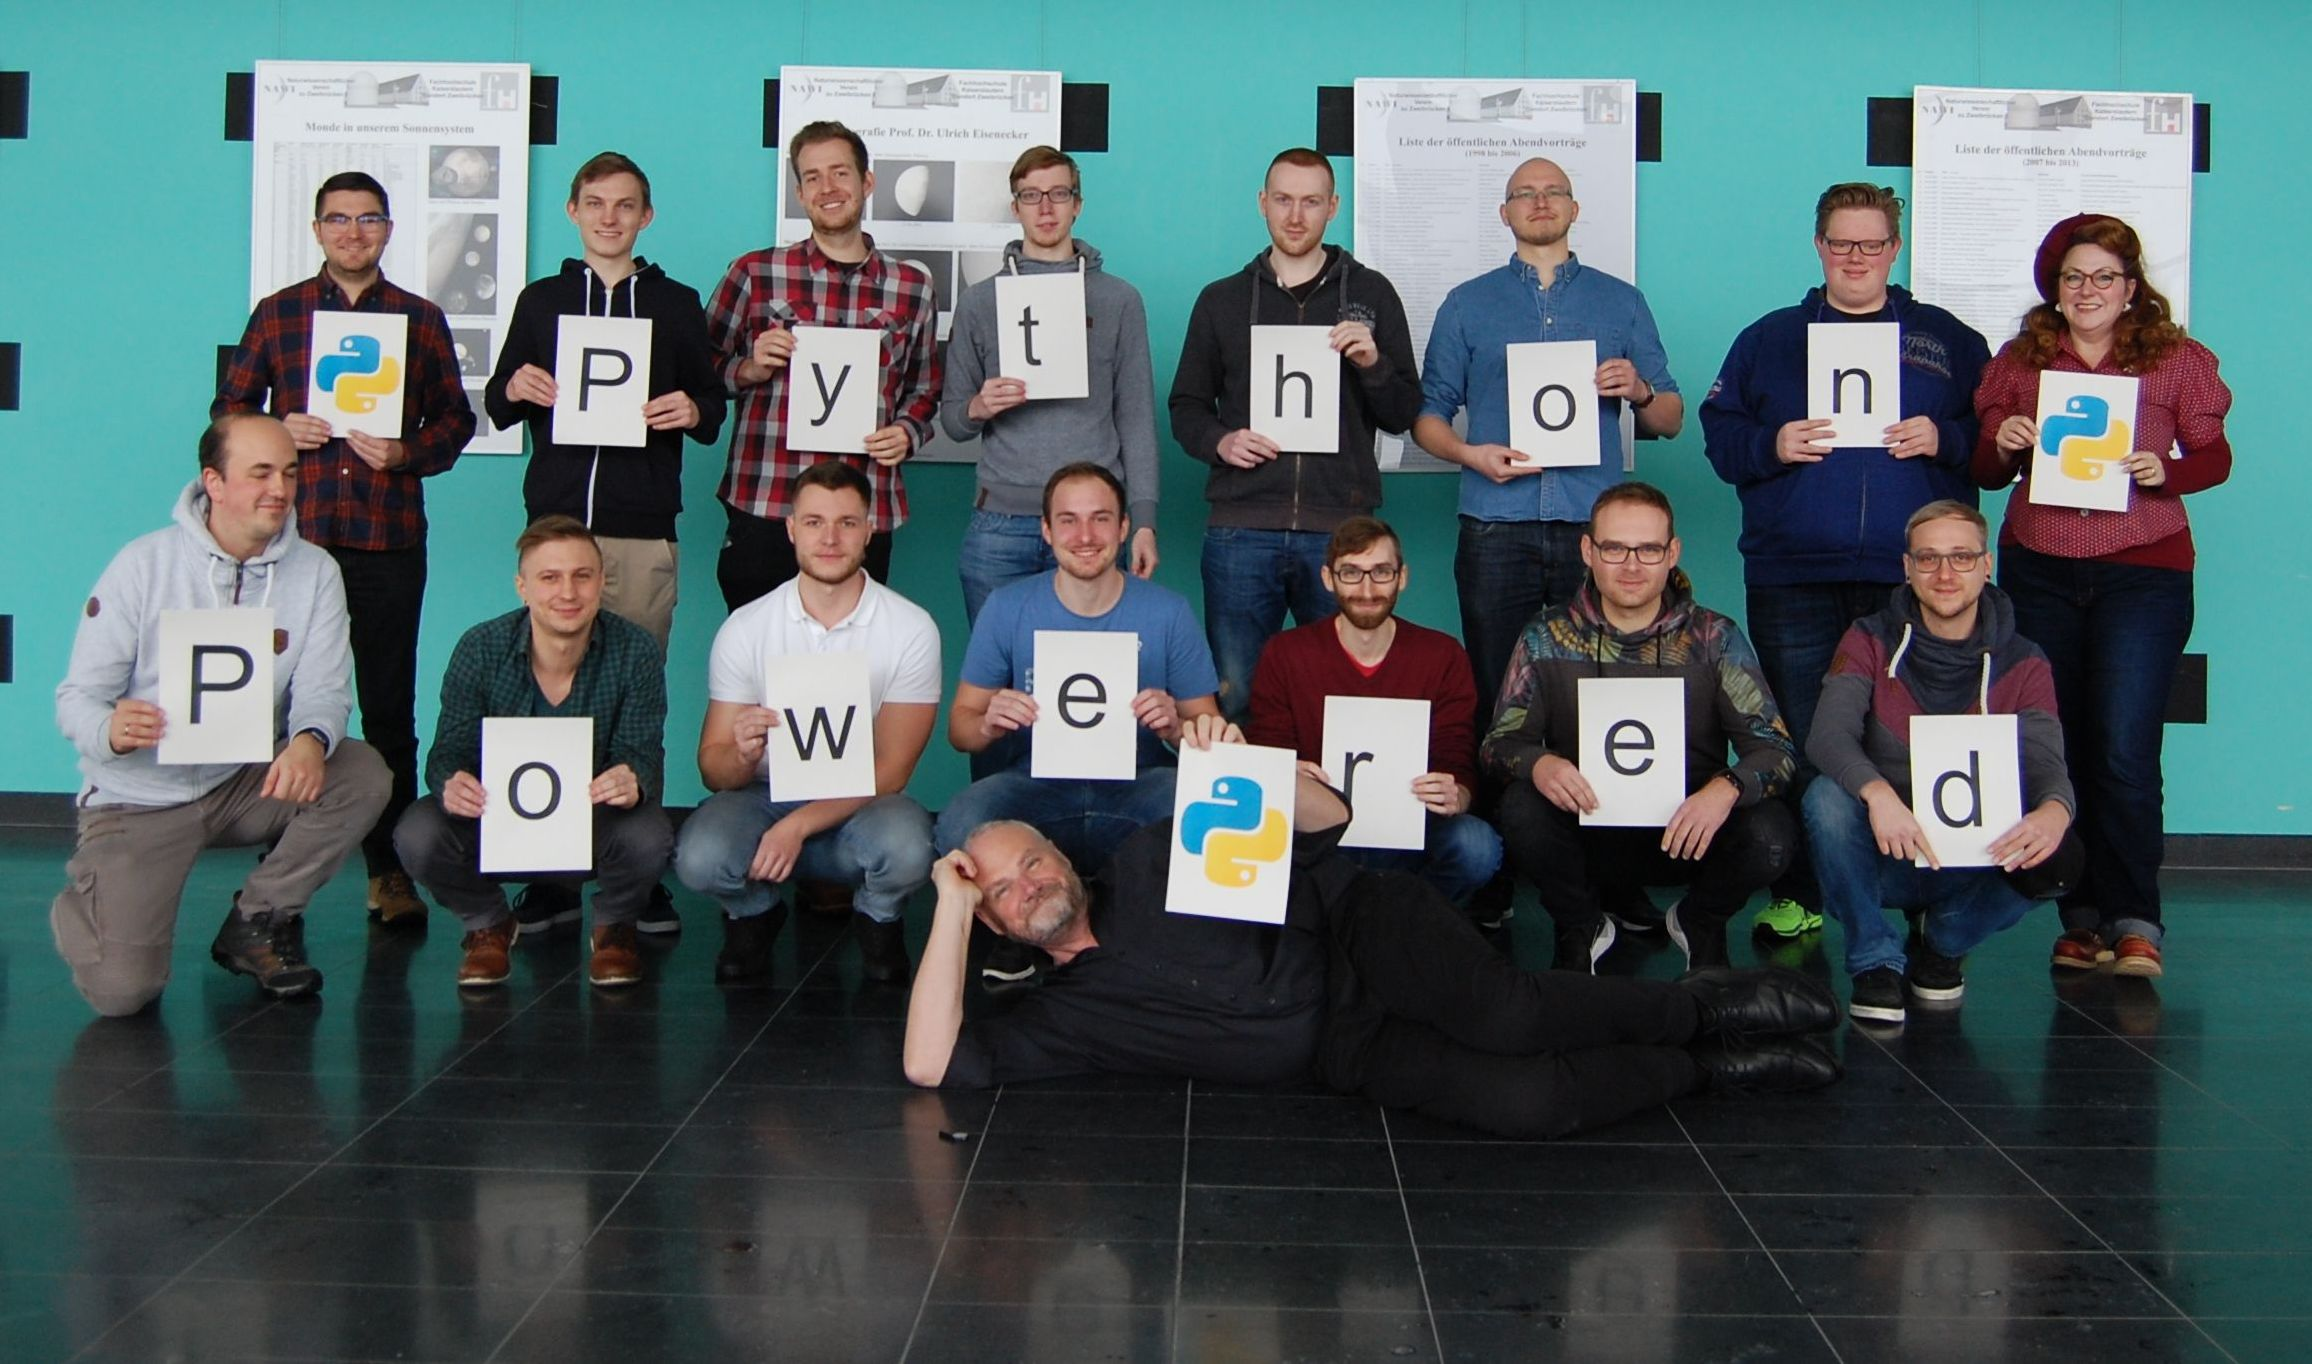
\includegraphics[width=\textwidth]{images/authors/theTeam}% Rotieren mit rotate=90
%\caption{\label{vorwort:team}Das Projektteam im Wintersemester 2018/19}
\end{figure}
\begin{tabular}{ll}
\centering
&Das Projektteam nach dem letzten Sprint Meeting\\
& im Januar 2019 von links nach rechts:\\
Hintere Reihe&Fabian Kalweit, Matthias Haselmaier, Marc Zintel,\\
                   &Robin Guth, Anatoli Sch�fer, Denis Schlusche,\\
                   &Kevin Konrad, Miriam Lohm�ller \\
Vordere Reihe&Mathias Fedder, Rainer Haffner, Lukas Kuhn,\\
                   &Sebastian Morsch, Julian Bernhart, Phillip Lauer,\\
                   &Christoph Seibel\\
Ganz vorne&Manfred Brill
\end{tabular}

\subsection*{Die studentischen Autoren}
Hier finden Sie nochmals die wichtigsten Personen in unserem Projekt, die studentischen Autoren mit Bild.
Es fehlen die Bilder von 
\begin{itemize}
\item Kevin Konrad
\item Denis Schlusche
\end{itemize}

\begin{table}
\centering
\begin{tabular}{p{5cm}|l}
Julian  Bernhart&
\includegraphics[width=3cm]{images/authors/bernhart}\\
Eric Brunk&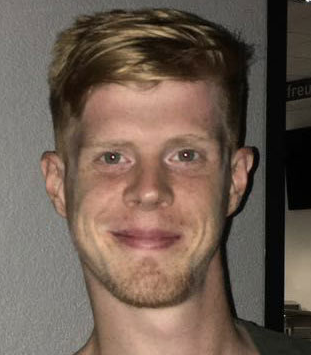
\includegraphics[width=3cm]{images/authors/brunk}\\
Mathias Fedder&
\includegraphics[width=3cm]{images/authors/fedder}\\
Robin Guth&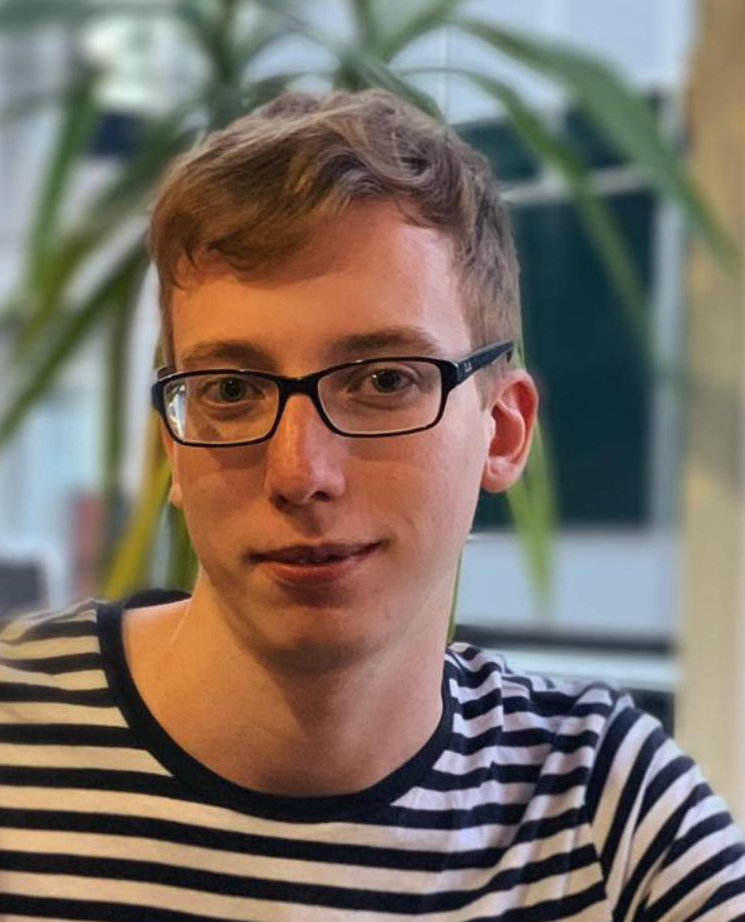
\includegraphics[width=3cm]{images/authors/guth}\\
Rainer Haffner&\includegraphics[width=3cm]{images/authors/haffner}\\
Matthias Haselmaier&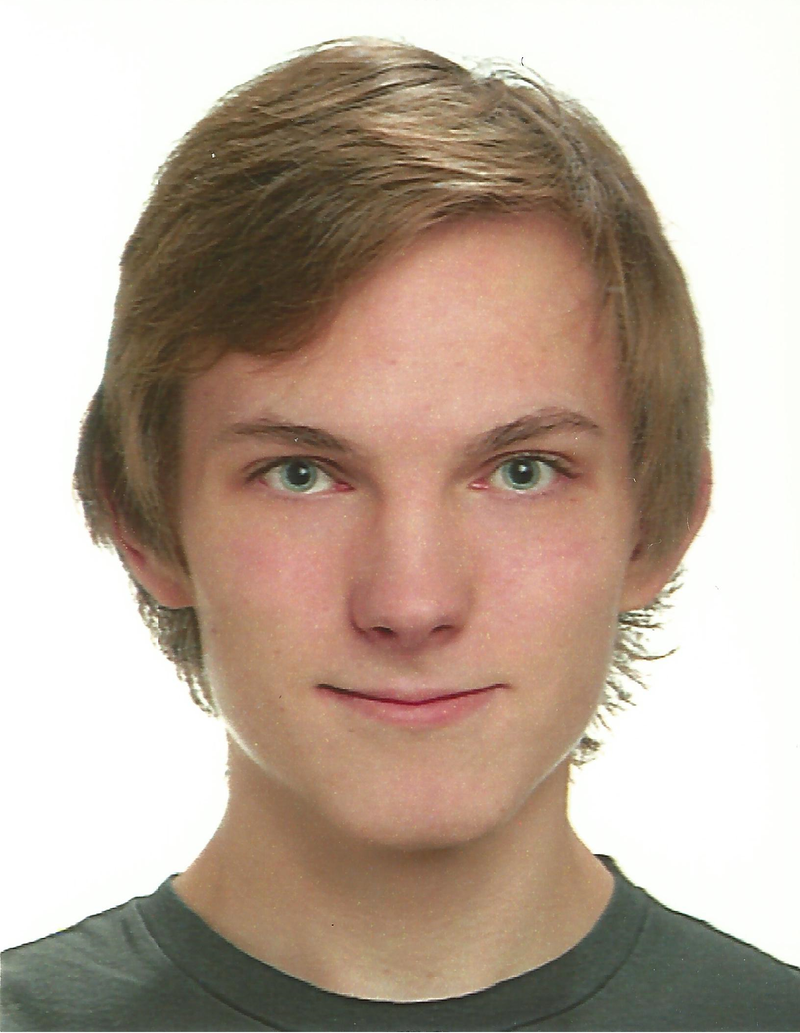
\includegraphics[width=3cm]{images/authors/haselmaier}
\end{tabular}
\end{table}
\pagebreak
\begin{table}
\centering
\begin{tabular}{p{5cm}|l}
Lukas Kuhn&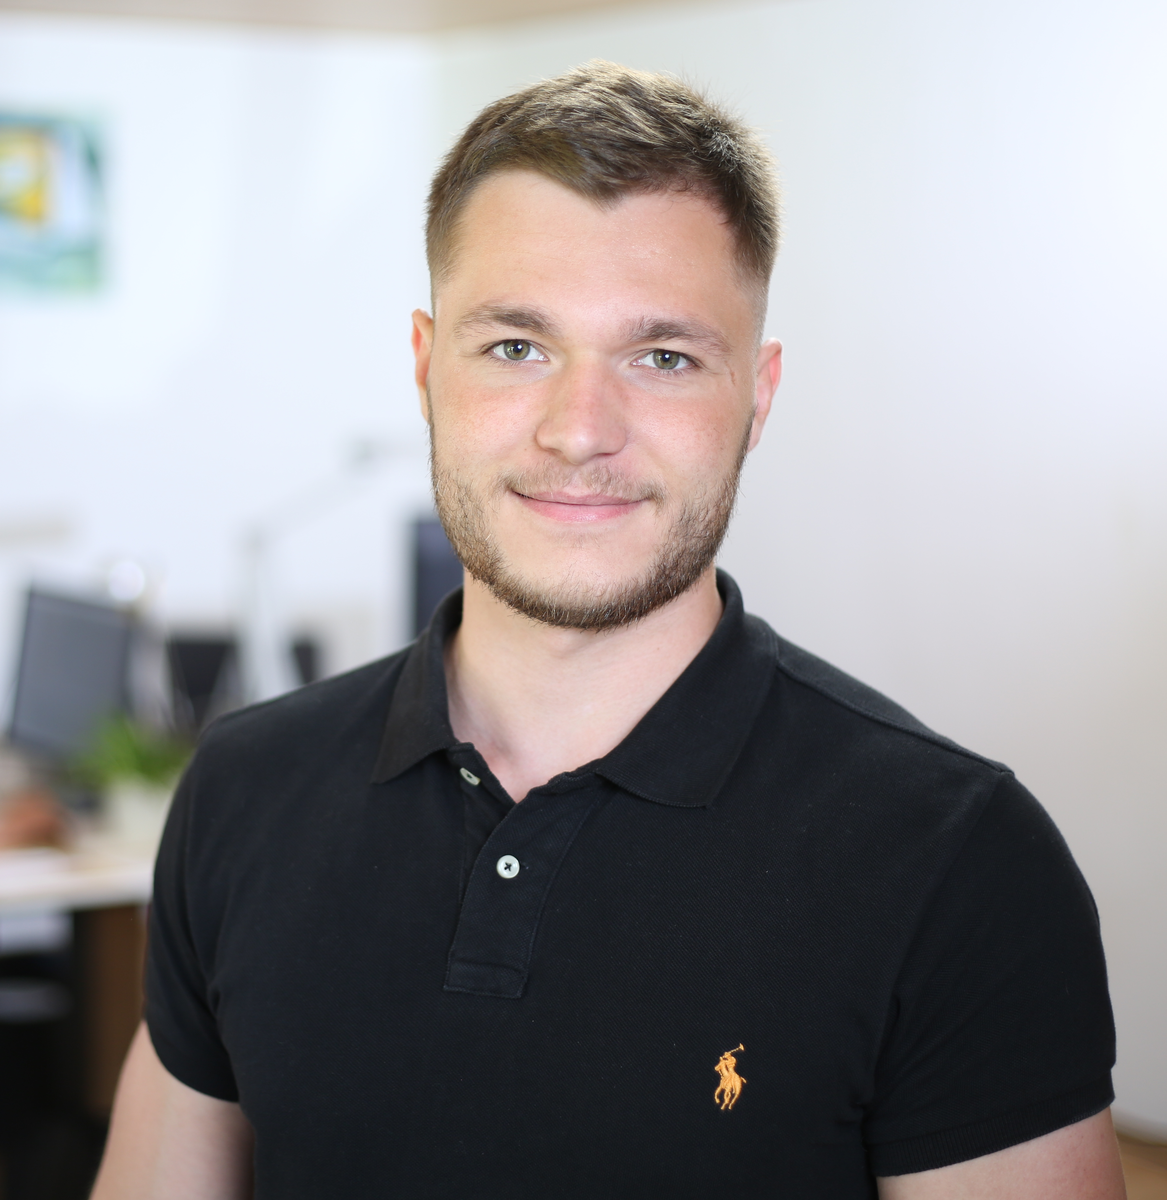
\includegraphics[width=3cm]{images/authors/kuhn}\\
Philipp Lauer&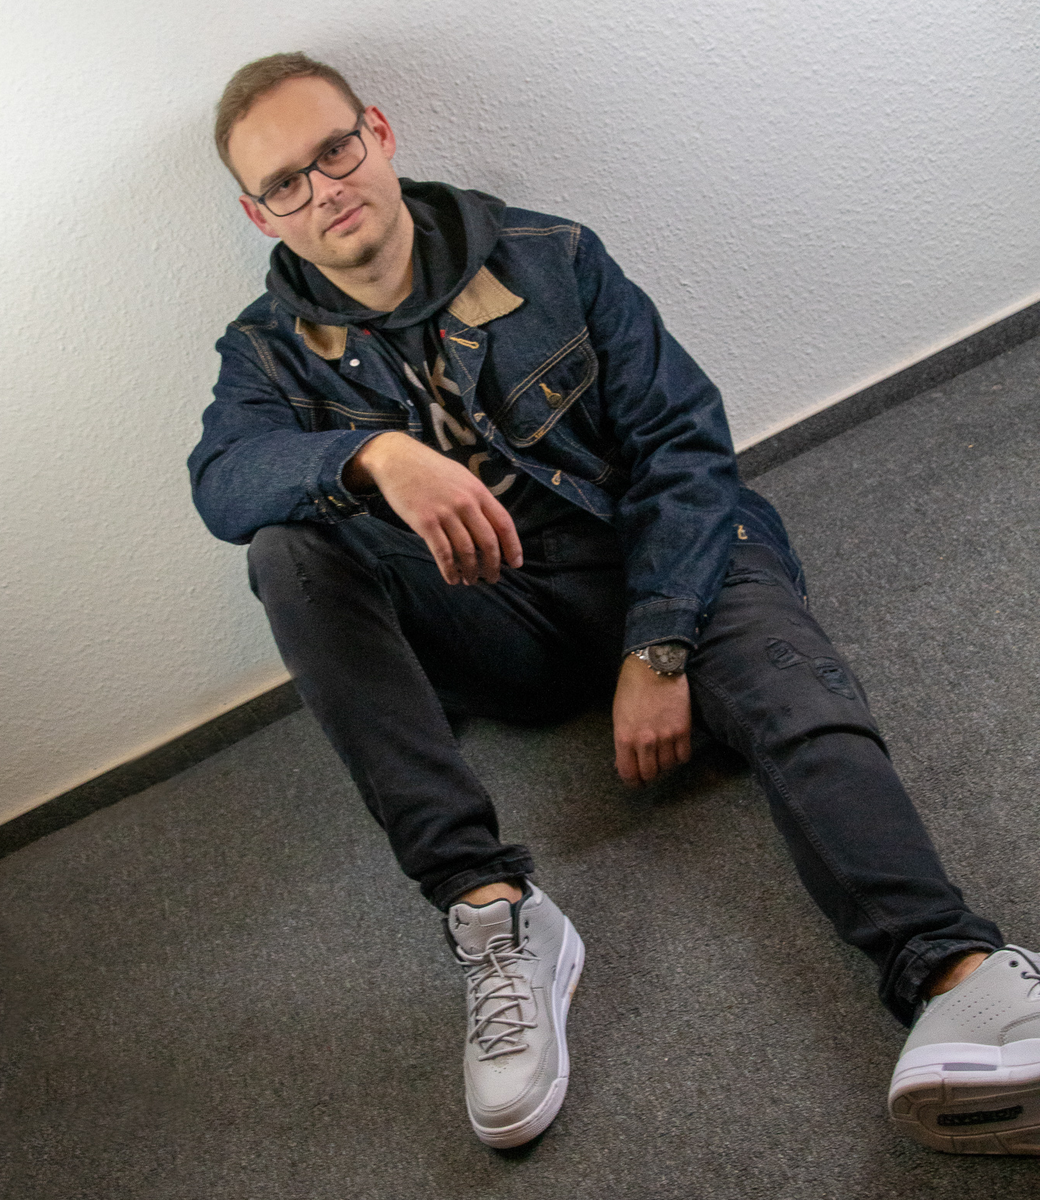
\includegraphics[width=3cm]{images/authors/lauer}\\
Sebastian Morsch&
\includegraphics[width=3cm]{images/authors/morsch}\\
Anatoli Sch�fer&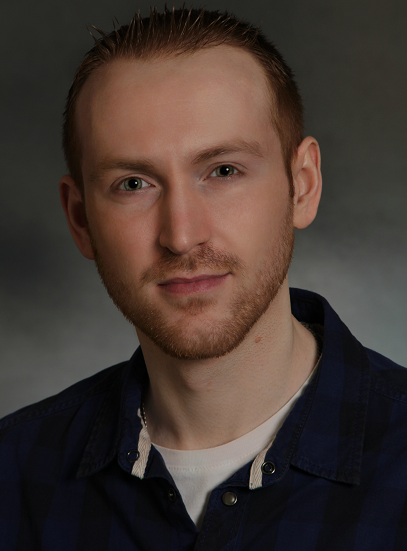
\includegraphics[width=3cm]{images/authors/schaefer}\\
Christoph Seibel&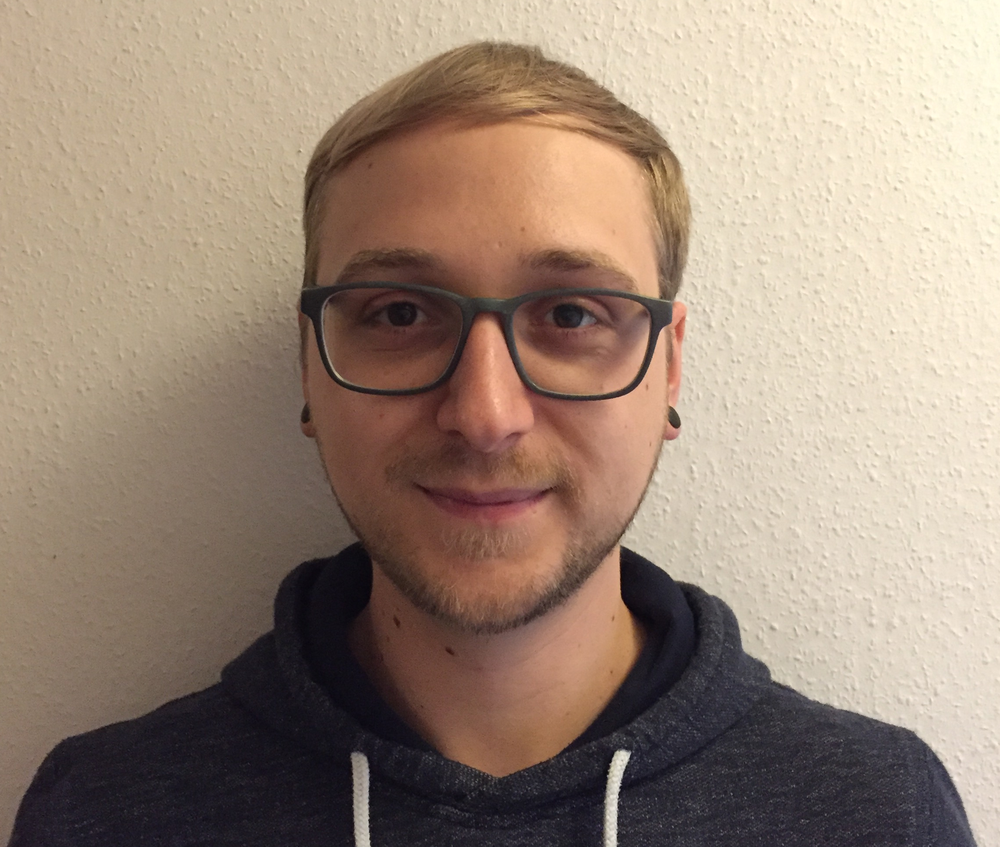
\includegraphics[width=3cm]{images/authors/seibel}\\
Marc Zintel&
\includegraphics[width=3cm]{images/authors/zintel}
\end{tabular}
\end{table}
%
\subsection*{Die Unterst�tzer}
Der erste Schritt zu diese Tutorial fand in der Lehrveranstaltung "`Aktuelle Themen aus Forschung und Praxis"'
des Masterstudiengangs "`Informatik"' im Fachbereich Informatik und Mikrosystemtechnik der Hochschule Kaiserslautern
statt. Eine Lehrveranstaltung in dieser Form mit einer sehr intensiven Betreuung konnte nur mit
einem Team bew�ltigt werden. Neben den Studierenden waren an diesem Projekt beteiligt:
\begin{itemize}
\item Miriam Lohm�ller --- Lektorat, Schreibstudio und Unterst�tzung im wissenschaftlichen Schreiben im Rahmen des Projekts "`InfoStuDi"' ("`Informatik studierenen in der digitalen Gesellschaft"'), gef�rdert vom Wissenschaftsrat.
\item Fabian Kalweit --- fachliches Lektorat, Administrator in GitHub, fachliche Betreuung als Assistent im Fachbereich Informatik und Mikrosystemtechnik.
    \item Manfred Brill --- Studiengangsleiter des Studiengangs "`Informatik"` und Projektleiter des Projekts "`InfoStuDi"'.
\end{itemize}

\begin{table}[ht]
\centering
\begin{tabular}{p{5cm}|l}
Miriam Lohm�ller&
\includegraphics[width=3cm]{images/authors/lohmueller}\\
Fabian Kalweit&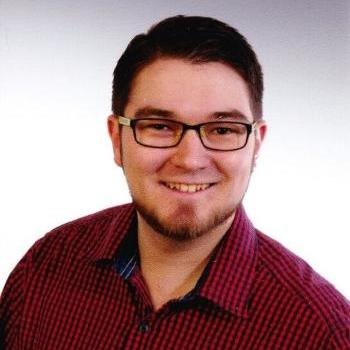
\includegraphics[width=3cm]{images/authors/kalweit}\\
Manfred Brill&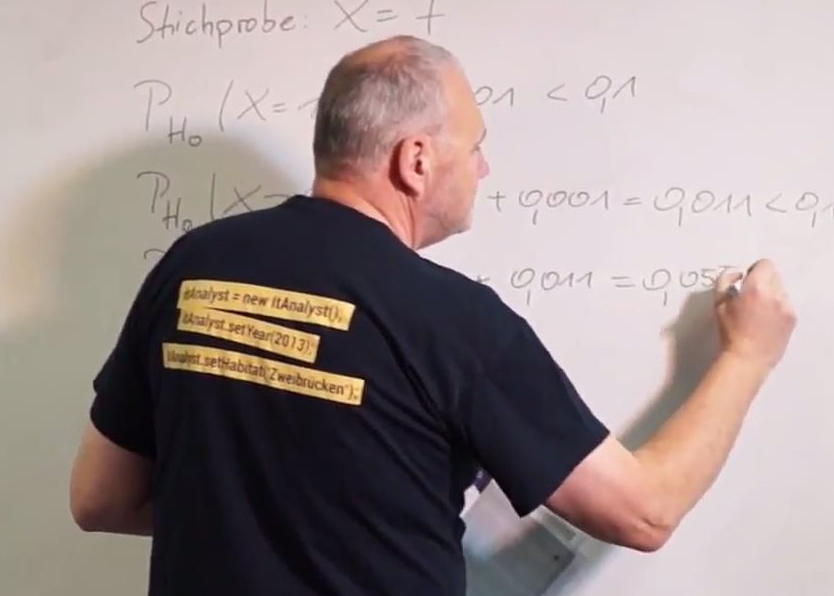
\includegraphics[width=3cm]{images/authors/brill}
\end{tabular}
\end{table}